% -----------------------------------------------------------------------------
% This source file is part of OSTIS (Open Semantic Technology for Intelligent Systems)
% For the latest info, see http://www.ostis.net
% 
% Copyright (c) 2012 OSTIS
% 
%
% OSTIS is free software: you can redistribute it and/or modify
% it under the terms of the GNU Lesser General Public License as published by
% the Free Software Foundation, either version 3 of the License, or
% (at your option) any later version.
% 
% OSTIS is distributed in the hope that it will be useful,
% but WITHOUT ANY WARRANTY; without even the implied warranty of
% MERCHANTABILITY or FITNESS FOR A PARTICULAR PURPOSE.  See the
% GNU Lesser General Public License for more details.
% 
% You should have received a copy of the GNU Lesser General Public License
% along with OSTIS.  If not, see <http://www.gnu.org/licenses/>.
% -----------------------------------------------------------------------------

\section{Введение}

\subsection{Что такое sc-код?}

\begin{frame}{Что такое семантическая сеть?}
  \textbf{Семантическая сеть} — информационная модель предметной
  области, имеющая вид графа, вершины которого соответствуют объектам
  предметной области, а дуги (рёбра) задают отношения между ними.
  \begin{figure}
    \centering
    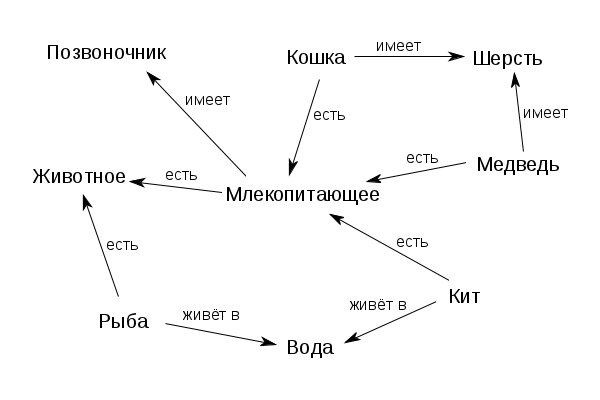
\includegraphics[scale=0.5]{intro/Semantic_net_example}
  \end{figure}
\end{frame}


\begin{frame}{Важные для нас особенности семантических сетей}
  Особенности семантических сетей:
  \begin{itemize}
  \item ориентированы на представление в смысловой части информации
  \item знак каждого объекта описываемой предметной области входит в
    семантическую сеть \textbf{однократно}
  \item каждый объект описываемой предметной области имеет
    неограниченное число связей с другими объектами этой области
  \end{itemize}
\end{frame}


\begin{frame}[shrink=10]{Что такое sc-код?}
  \textbf{SC-код} (Semantic Code, абстрактный семантический
  компьютерный код) — универсальный язык бинарных семантических сетей.
  
  Для подачи человеку существует строковая форма SCs (SC string),
  графическая форма SCg (SC graphical), естественноязыковая SCn (SC
  natural). В этой презентации я буду использовать SCg:
  \begin{figure}
    \centering
    \includegraphics[scale=0.45]{intro/SC_code_example}
  \end{figure}
\end{frame}

\begin{frame}[shrink=5]{Текст на SC-коде}
  Семантическая сеть в SC-коде называется \textbf{sc-текстом}
  (\textbf{sc-конструкцией}).  Ниже приведен sc-текст
  (sc-конструкция). Любой элемент в sc-тексте называется
  \textbf{sc-элементом}. SC-текст хранится в специальной памяти -
  \textbf{sc-памяти.}

  \begin{figure}
    \centering
    \includegraphics[scale=0.55]{intro/SC_code_example}
  \end{figure}
\end{frame}

\begin{frame}{Узлы sc-конструкции}
  Узел в sc-конструкции называется \textbf{sc-узлом} и бывает
  различных видов.
  
  \begin{figure}
    \centering
    \includegraphics[scale=0.55]{intro/SC_code_example_nodes}
  \end{figure}
\end{frame}

\begin{frame}[shrink=5]{Связи в sc-конструкции}
  Связь в sc-конструкции в общем случае называется \textbf{sc-коннектором},
  который бывает неориентированным (\textbf{sc-ребро}) и ориентированным
  (\textbf{sc-дуга}).
  
  \begin{figure}
    \centering
    \includegraphics[scale=0.55]{intro/SC_code_example_connectors}
  \end{figure}
\end{frame}

\begin{frame}[shrink=5]{SC-код и теория множеств}
  SC-код основан на теории множеств, поэтому все sc-узлы обозначают
  либо внешние объекты по отношению к sc-памяти, либо sc-множества, а
  sc-коннекторы обозначают связки отношений.
  
  \begin{figure}
    \centering
    \includegraphics[scale=0.55]{intro/SC_code_example}
  \end{figure}
\end{frame}

%%% Local Variables: 
%%% mode: latex
%%% TeX-master: "sc_code_in_examples"
%%% End: 
